%! TEX root = ../notes/main_notes.tex

\lecture{Introduction to the Course}{lec-01}

% Only appears in book/notes mode
\mode<article>{
	\section{Overview \& Objectives}
	The term \emph{sustainability} implies continuity and balance.  If something is sustainable, it can continue doing what it is doing.  Unless it is doing nothing, what it is doing is interacting with other entities.  This implies that, except for those things that are doing nothing, we should think about sustainability with a systems perspective.
	
	A system is a collection of entities (or elements) and the connections between them.  To understand a system, we need to understand the entities and their connections.  Our goal in this course is to develop an understanding of the relationship between the economy and the environment by looking at the elements that make up the economy and their relationship with elements that make up the environment.  To do so, we will proceed by building a model of a \emph{complex adaptive social ecological system}. 
	
	The system we inhabit, and that we will try to understand, is complex.  This means that the system as a whole exhibits properties that cannot be explained by looking at any element itself.  It is adaptive in that it changes in response to internal and external pressures.
	
	\begin{note}
		Key reading for this section: Chapter 1 of the required textbook.
	\end{note}
}

% Frame 1

\begin{frame}{Systems}
	% \begin{columns}
		% \column{0.6\textwidth}
			\begin{itemize}
				\item A system is a collection of elements and their connections.
				\item A social ecological system contains elements in both the social (human) and ecological (nature) domains, and has connections crossing between the domains.
				\item A system is complex when there are 'emergent' properties that cannot be predicted looking at elements in isolation.
				\item A system is adaptive if it continuously evolves or changes in response to internal and external forces.
			\end{itemize}
		% \column{0.4\textwidth}
		% 	\centering
		%	\includegraphics{SESgraphic.png}
	% \end{columns}
\end{frame}

\begin{frame}{Systems}
	\centering
	\includegraphics<presentation>[width=0.6\linewidth]{SESgraphic.png}
	\includegraphics<article>[width=0.8\linewidth]{SESgraphic.png}
\end{frame}


% Interspersed notes text between slides
\mode<article>{
	\subsection{Systems and Subsystems}
	The global social ecological system is far too complex for anyone to comprehend.  At present, it is probably too complex for AI to comprehend as well.  What both humans and AI do with this is focus on a part of the system that we are interested in.  We choose a boundary and a scale.  Things beyond the boundary are grouped together into subsystems, the internal details of which are not considered.  This would be at the scale that is coarser than the part of the system we are interested in.  For those things at a finer scale, we also relegate those things into subsystems, with the entire subsystem being taken as an element of the system we are studying.
	
	The concerns about sustainability can be seen as concerns about the details that are being left out.
	
	
}

\begin{frame}{Production Possibilities}
	\begin{columns}[T]
		\begin{column}{0.3\textwidth}
			\begin{itemize}
				\item What is missing?
			\end{itemize}
		\end{column}
		\begin{column}{0.7\textwidth}
			\centering
			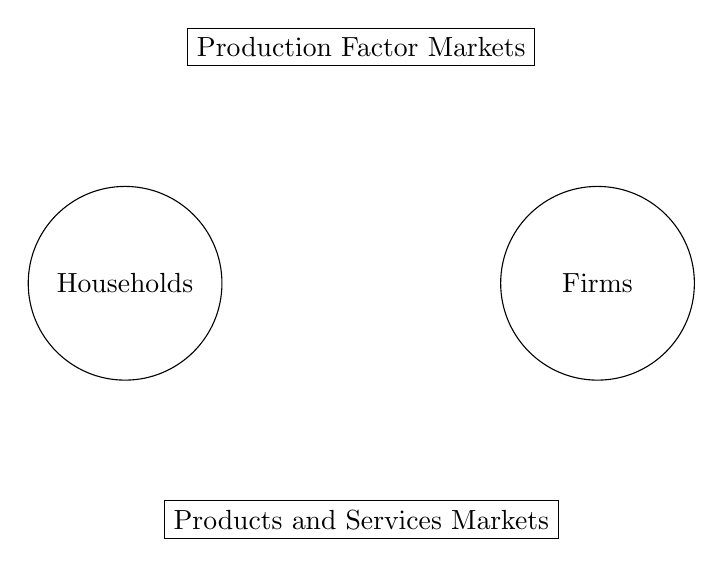
\begin{tikzpicture}
				\node [rectangle, draw] at (3,6) {Production Factor Markets};
				\node [rectangle, draw] at (3,0) {Products and Services Markets};
				\node [circle, draw, minimum size=70pt] at (0,3) {Households};
				\node [circle, draw, minimum size=70pt] at (6,3) {Firms};
			\end{tikzpicture}
		\end{column}
	\end{columns}
\end{frame}
